\clearpage
\section{A-star search}
\subsection{Basic Idea}

A* is a kind of informed search, which is different from traditional uninformed search (such as bfs). One huge difference is, instead of searching while trying to maintain as least cost as possible in bfs, A* also consider anohter value called heuristic. Figure \ref{astar} is a demostration of A* algorithm. On one hand, the solid line represent the path that we alredy go through, which is an evaluation of the past. On the other hand, the dash line, it represents the estimated/expected cost from current state to the goal, which is an evaluation of the future.

At every time A* pick the new state with lowest priority from a priority queue. Usually, it considers the past and the future simultaneously. Let's say the priority value is $f$, value of cost is $g$, and heuristic is $h$, then:
$$f = g + h$$

\begin{figure*}[!h]
\centering
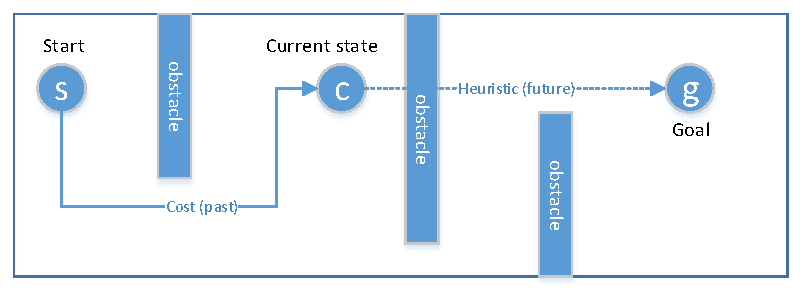
\includegraphics[width=0.927\textwidth]{astar.pdf}
\caption{A demostration of A* algorithm}
\label{astar}
\end{figure*}



\subsection{Single robot problem model}
The basic idea of single robot is to find a path from start position to the goal position. The state here is the coordinate of the robot, $(x,y)$.




\subsection{Code implementation}
\textbf{Line 3-7:} There are three major data structure to help me code astar.
\begin{itemize}
\item Priority queue: I use a priority queue to store the \emph{frontiers}, sorted by prioirty. Every search I will pop a node from the head of the queue.
\item Hash Map $\times 2$: One hashmap maps from node to node, for creating a backchain at the end. Another hashmap maps from node to priority, for the situation when we re-visit a node, it only worth expanding only if it has higher priority/cost than before.
\end{itemize}

\begin{lstlisting}[numbers=left]
public List<SearchNode> astarSearch() {
  resetStats();
  // implementing priority queue for the frontiers
  PriorityQueue<SearchNode> frontiers = new PriorityQueue<>();
  // implementing hashmap for the chain and the visited nodes
  HashMap<SearchNode, SearchNode> reachedFrom = new HashMap<>();
  HashMap<SearchNode, Double> visited = new HashMap<>();

  // initiate the visited with startnode
  reachedFrom.put(startNode, null);
  // initiate the frontier
  frontiers.add(startNode);
  while (!frontiers.isEmpty()) {
    // keep track of resource
    updateMemory(frontiers.size() + reachedFrom.size());
    incrementNodeCount();
    // retrieve from queue
    SearchNode current = frontiers.poll();
    // discard the node if a shorter one is visited
    if (visited.containsKey(current)
        && visited.get(current) <= current.priority())
      continue;
    else
      visited.put(current, current.priority());
    // mark the goal
    if (current.goalTest())
      return backchain(current, reachedFrom);
    // keep adding the frontiers and update visited
    ArrayList<SearchNode> successors = current.getSuccessors();
    for (SearchNode n : successors) {
      if (!visited.containsKey(n) || visited.get(n) > n.priority()) {
        reachedFrom.put(n, current);
        frontiers.add(n);
      }
    }
  }
  return null;
}
\end{lstlisting}

\textbf{Line 20-28:} After poping the node, we check for two condition. One is if it is the goal, we simply return the solution path and terminate the search. Antoher condition is, if the node has been visited before, we don't push it into \emph{frontiers} unless it has shorter cost than before.

\textbf{Line 29-35:} Get the successors of currrent node, and push those un-visited nodes or node has shorter cost than before, into the \emph{frontiers}.



\subsection{Output demonstration}



I use Simplex Noise to generate the maze.\footnote{I use authoried code from \url{http://webstaff.itn.liu.se/~stegu/simplexnoise/SimplexNoise.java to help me with the noise}} Figure \ref{s-1} shows a $40\times40$ maze, where all three robots try to move from bottom-left to middle-right. I leave the direction of robot at every single node. You can see that bfs and A* perform quite almost equally well, while dfs goes through a lengthy path.

The following output shows that, A* explored significantly less node than bfs, while the path length (cost) almost as less as bfs, while comparing to dfs.



\begin{lstlisting}[numbers=left]
BFS:
Nodes explored during search: 1064
Maximum space usage during search 1099
path length: 60
DFS:
Nodes explored during search: 399
Maximum space usage during search 242
path length: 242
A*:
Nodes explored during search: 79
Maximum space usage during search 224
path length: 72
\end{lstlisting}


\begin{figure*}[!h]
\centering
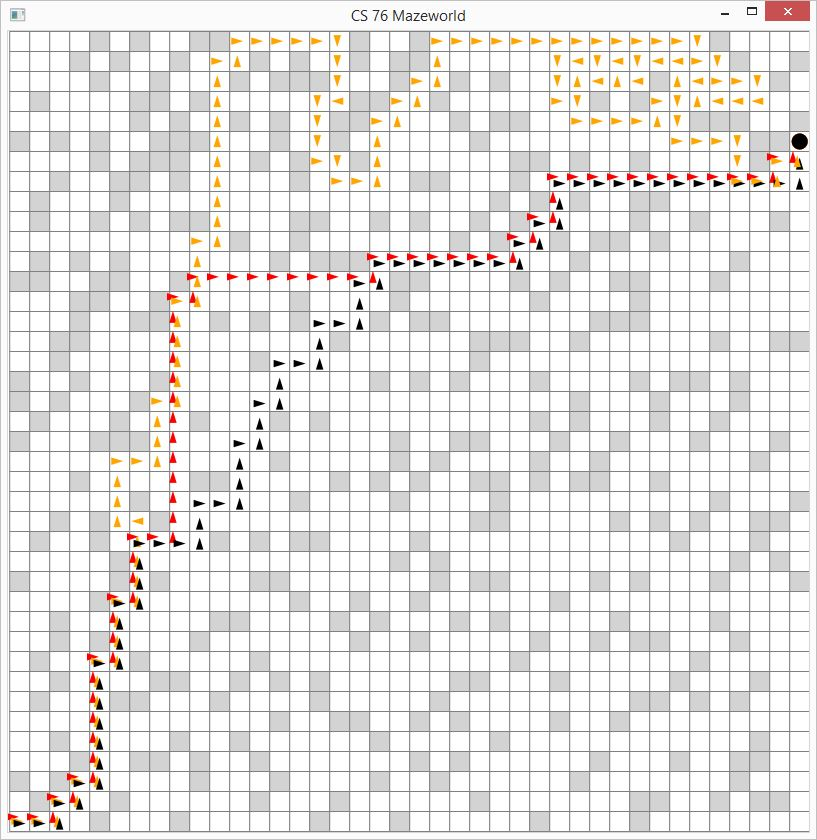
\includegraphics[width=0.618\textwidth]{s-1-1.JPG}
\caption{Searhing path of dfs(orange), bfs(red) and A*(black)}
\label{s-1}
\end{figure*}




\subsection{Discussion on cost and heuristic}
A* leverage both the cost (penalty) and the heuristic (search speed). Currently we use $f = h + g$ for priority, which seems quite a balanced solution. What happens if we go to extrem where the priority only related to $g$ or $h$? Or, is 50:50 the best choice for $f$?

Before I begin to discuss, I want to introduce a new kind of maze, where the obstacles can be crossed, while there is a certain amount of penalty. While I am first use Simplex Noise generate a maze, i replace the wall with number ranging from 1 to 10 to represent the weights. I use the following functions to differentiate nodes with different weights.
$$Grayscale = 255 - 255 \times weight / 20$$

Here I modify the expression of priority as following:
$$f = \alpha \cdot h + (1 - \alpha ) \cdot g$$
Then I vary $\alpha$ from 0 to 1, and observe their path length and cost. Figure \ref{s-2} shows the visual path with different configuration.
\begin{itemize}
\item Red ($\alpha = 0.0$) is an extreme case when A* only considers the cost, and becomes uninformed search. (I think it act like Dijkstra Algorithm). Since we are using Manhattan distance and the goal is at top-right, every action of moving south or west is a compromise of cost, and neglecting of path length ( search speed).
\item Brown ($\alpha = 1.0$) is another extreme case when A* only considers the heuristic, and becomes best-first search. We can observe that it totally neglect the cost/penalty, rushing to the goal in the simplest path.
\end{itemize}

Figure \ref{gh-plot} shows the change of path length and cost while varying $\alpha$. It depends on the tradeoff on searching speed and cost. It also greatly related to the problem definition, which affects the apperance of state space. For example, if path length and cost are on the scale $a : b$, then we should find $\alpha$, s.t. $min(a \cdot cost + b \cdot length)$.

\begin{figure*}[!h]
\centering
\includegraphics[width=0.628\textwidth]{astar_alpha.eps}
\caption{Plot describes the relationship between cost, path length, and $\alpha$}
\label{gh-plot}
\end{figure*}

\begin{figure*}[!h]
\centering
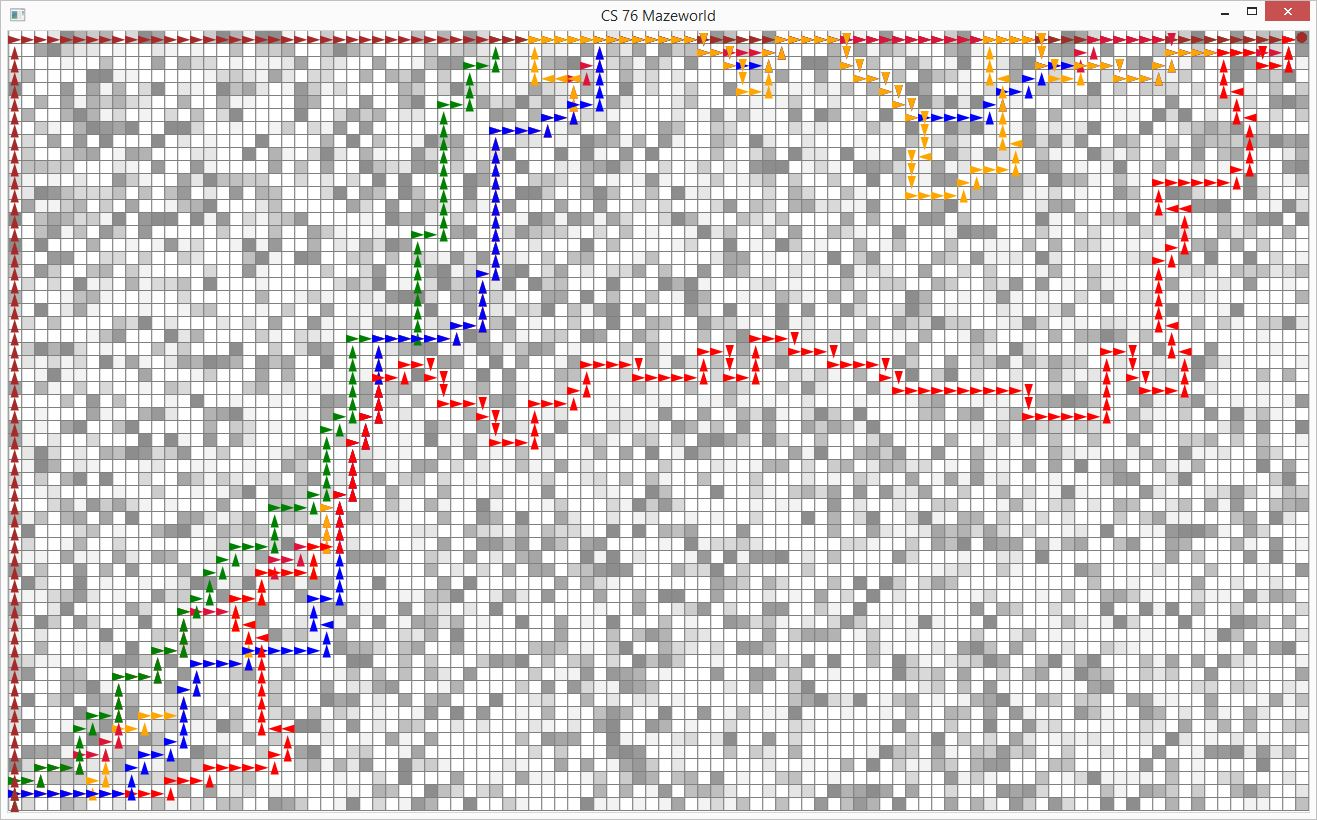
\includegraphics[width=1\textwidth]{s-2-1.JPG}
\caption{Varying the $\alpha$ in A* as 0.0 (red), 0.25 (orange), 0.5 (blue), 0.75 (crimson), 0.9 (green), 1.0 (brown)}
\label{s-2}
\end{figure*}

